
\documentclass[12pt]{article}
\usepackage[a4paper]{geometry}
\usepackage[myheadings]{fullpage}
\usepackage{fancyhdr}
\usepackage{lastpage}
\usepackage{graphicx, wrapfig, subcaption, setspace, booktabs}
\usepackage{amsmath}
\graphicspath{ {./images/} }
\usepackage[T2A]{fontenc}
\usepackage[utf8]{inputenc}
\usepackage[font=large, labelfont=bf]{caption}
\usepackage{fourier}
\usepackage[protrusion=true, expansion=true]{microtype}
\usepackage[english,russian]{babel}
\usepackage{sectsty}
\usepackage{url, lipsum}

    \usepackage{array}
    \newcolumntype{C}[1]{>{\centering\arraybackslash}p{#1}}

\pagestyle{empty}

\begin{document}

\begin{center}
\normalsize{Минестерство образования и науки Российской Федерации}\\
\normalsize{Федеральное государственное бюджетное образовательное}\\ 
\normalsize{учреждение высшего профессионального образования}\\
\normalsize{{Нижегородский государственный университет им. Н.И. Лобачевского}}\\
\hfill \break
\normalsize{{Институт информационных технологий, математики и механики}}\\
\end{center}
\vfill
\begin{center}
\hfill \break

\Large
{
\textbf{Отчет по лабораторной работе}
\linebreak
Управление скоростью вращения DC-моторамотора
}
\end{center}
\vfill


\begin{flushright}
\large{
Выполнили студенты группы 381503-3\\
Конаков А.В.\\
Косоруков О.Д.\\
}

\end{flushright}


 
\vfill
\begin{center} 
Нижний Новгород\\ 2018 
\end{center}
\pagebreak






\newpage
\tableofcontents
\newpage

%\sectionfont{\scshape}







\section*{Введение}
\addcontentsline{toc}{section}{Введение}
\paragraph{}
В современном мире DC-моторы используются повсеместно: вмоторы используются повсеместно: в
аккумуляторных инструментах (дрели, шуруповерты)
компьютерной технике, бытовых электроприборах
(стиральные машины, холодильники, вентиляторы,
пылесосы), игрушках, р/у моделях, робототехнике, станках,
промышленных приборах, электромобилях и прочей технике.
Чтобы разрабатывать, создавать, модифицировать и
использовать такие устройства важно понимать, как именно
устроен DC-моторы используются повсеместно: вмотор, принцип его работы и происходящие
процессы.\hfill
\paragraph{}
Для функционирования большинства современных
механизмов, в которых используется электромоторы
безусловно существует проблема регулирования и
стабилизации скорости. Она решается при помощи систем с
контуром обратной связи, в который входят датчики, дающие
информацию о скорости вращения. Стабилизация скорости
осуществляется специальными регуляторами. Обычно
применяются пропорционально-моторы используются повсеместно: винтегрально-моторы используются повсеместно: в
дифференциальные (ПИД) регуляторы, как более
универсальные, или пропорционально-моторы используются повсеместно: винтегральные (ПИ),
как более простые. Сложность расчета и исполнения
обусловлена тем, что приходится учитывать не только тип
двигателя, но и всю систему привода в целом. Из-моторы используются повсеместно: вза этого
характеристики регулирования в данных системах
определяются экспериментально.
\vfill
\newpage






\section*{Цель работы}
\addcontentsline{toc}{section}{Цель работы}
\paragraph{}
Исследовать вопросы обеспечения заданного качества
протекания переходных процессов. Рассмотреть физическую
и математическую модели DC-моторы используются повсеместно: вмотора. Построить
математическую модель объекта управления. Исходя из вида
полученной модели и значения ее параметров разработать
системы управления, обеспечивающие поддержание
заданного закона изменения скорости вращения или
углового положения вала DC-моторы используются повсеместно: вмотора. Сопоставить поведение
математической модели с поведением моделируемого
(реального, физического) устройства.
\vfill
\newpage










\section*{Математическая модель}
\addcontentsline{toc}{section}{Математическая модель}
\paragraph{}
Объектом управления в данной работе является DC-моторы используются повсеместно: вмотор.
Построим его математическую модель, опираясь на
представления о его физическом устройстве,
проиллюстрированном на Рис.1.

\begin{figure}[h]
	\centering
	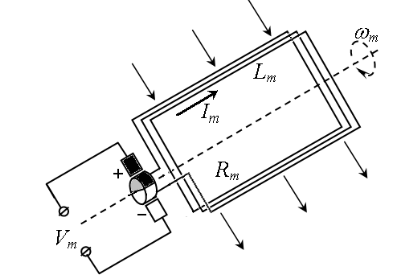
\includegraphics[scale=0.5]{motorabstract}
	\caption[0.5\textwidth]{Устройство электрической части электромотора постоянного тока}
\end{figure}

\paragraph{}
DC-моторы используются повсеместно: вмотор имеет как электрические, так и механические
свойства. Рассматривая мотор как механическую систему
необходимо учесть, что в его корпусе есть вращающийся
ротор, общий момент инерции которого с учетом
инерционности массивного диска, насаженного на вал
ротора, составляет величину $J_{eq}$ . Обмотка ротора
представляет собой катушку с индуктивностью $L_m$ и
омическим сопротивлением $R_m$ , вращающуюся вместе с
ротором в магнитном поле статора. Напряжение $V_m$ на
катушку подается через скользящие контакты коллектора.
Протекающий в обмотке ток $I_m$ , взаимодействуя с
магнитным полем статора, создает вращающий момент $\mu_m = K_tI_m$, действующий на ротор. При составлении уравнений
следует также учитывать эффект наведения дополнительной
электродвижущей силы (ЭДС) в обмотке ротора за счет
вращения с угловой скоростью $\omega_m$ его катушки-моторы используются повсеместно: вобмотки в
магнитном поле статора. Величина этой ЭДС
пропорциональна скорости вращения с неким
коэффициентом и составляет $K_m \omega_m$.

\paragraph{}
Уравнения, приближенно описывающие закон изменения
тока в обмотке ротора для разомкнутой системы управления
DC-мотором могут быть записаны в следующем виде:
$I_m R_m =V_m(t)-\varepsilon_m$ , $\varepsilon_m = K_m\omega_m$,
где $\varepsilon_m = K_m\omega_m$ – наводимая в обмотке ротора ЭДС индукции
(за счет вращения катушки в магнитном поле статора).
\paragraph{}
Уравнения для механической части мотора,
приближенно описывающие динамику вращения его ротора
(без учёта сил трения) имеют вид: 
$J_{eq}\frac{d}{dt}\omega_m =\mu_m$, $\mu_m = K_t I_t$,
где величина $\mu_m$ определяет вращающий момент,
действующий на обмотку ротора.\hfill\break
Модель электромотора, в целях дальнейшего исследования,
удобно представить через его коэффициент передачи (от входного 
напряжения к скорости углового вращения), используя изображения по Лапласу.
Коэффициент передачи описывает (в изображениях) связь вида: $\omega(s) = K(s)V(s)$.

\paragraph{}
Из предыдущих получаем выражение для $K(s)$: $K(s) = \frac{K_t}{R_mJ_{eq}+K_tK_m}$. который может быть представлен в виде
произведения постоянное коэффициента усиления $a = \frac{1}{K_m}$ на типового инерционного звена $W(s) = \frac{1}{Ts+1}$, где $T = \frac{R_mJ_{eq}}{K_tK_m}$, т.е. получим $K(s) = \frac{a}{Ts+1}$

\paragraph{}
Подадим на вход мотора напряжение, изменяющееся
скачком от нуля до 1В (т.е. функцию Хевисайда). Оригинал
этого отклика (обозначим его $h(t)$) может быть легко
вычислен. При t > 0: 
$h(t) = a(1 - e^{-tT})$.
Рассмотрим реакцию системы на импульс напряжения $u^*$
подаваемый на отрезке $[t_1 , t_2 ]$:
$u^* = (\eta(t - t_1) - \eta(t - t_2))$ и
$\eta(t-t_0) = \frac{e^{-pt_0}}{s}$\hfill\break
$\frac{au^*(e^{-pt_1} - e^{-pt_2})}{s(Ts+1)} = 
au^*(e^{\frac{t_2 - t}{T}}\eta(t - t_2) - 
     e^{\frac{t_1 - t}{T}}\eta(t - t_1))+ 
(\eta(t - t_1) - \eta(t - t_2))$

\[
\omega_m(t) = 
\begin{cases}
  0,  & \textit{если}\quad t < t_1\\
  \frac{1}{K_m}(1 - e^{\frac{K_tK_m}{J_{eq}R_m}(t_1 - t)}), & \textit{если}\quad t_1 \leqslant  t < t_2 \\
  \frac{1}{K_m}(e^{\frac{K_tK_m}{J_{eq}R_m}(t_2 - t)} - e^{\frac{K_tK_m}{J_{eq}R_m}(t_1 - t)}), & \textit{если}\quad t \geqslant  t_2
\end{cases}
\]
\paragraph{}
Графически переходной процесс представлен на Рис.2. %по нормальному лучше на ссылку заменить
\begin{center}
	

\begin{figure}[h]
\centering	

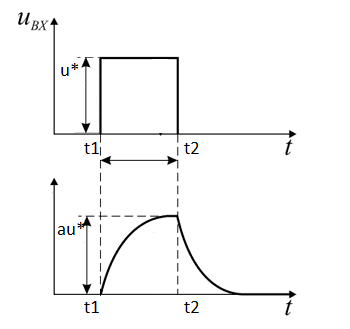
\includegraphics[scale=0.6]{impulse}
\caption{Отклик системы на импульс длины $t_1 - t_2$}
\end{figure}
\end{center}
\vfill
\newpage






\section*{Экспериментальное исследование
процессов управления реальным объектом}
\addcontentsline{toc}{section}{Экспериментальное исследование
процессов управления реальным объектом}
\paragraph{}
Работа будет выполняться на экспериментальной установке DC-мотор. В её состав входят
DC-моторы используются повсеместно: вмотор. В ее состав входят:
\begin{itemize}
	\item  компьютер с установленной средой LabView и встроенной DAQ-картой
	\item рабочая станция NI-моторы используются повсеместно: в ELVIS
	\item физический прибор QNET DC Motor Control Trainer (DC-мотор с датчиками поворота, скорости вращения, силы тока и массивный диск)
\end{itemize}
Будет использоваться программа-моторы используются повсеместно: ввиртуальный прибор
$QNET\_DC\_Motor\_Lab\_01\_speed\_control.vi$


\vfill
\newpage








\section*{Идентификация параметров DC-моторы используются повсеместно: вмотора}
\addcontentsline{toc}{section}{Идентификация параметров DC-моторы используются повсеместно: вмотора}
\paragraph{}
Оценим параметры $R_m$ и $K_m$. Для этого будем изменять напряжение с шагом 1В, начиная от -5В и заканчивая 5В. На каждом шаге измерим скорость мотора $\omega_m$,
ток, протекающий в обмотке ротора мотора при его вращении $I_m$, и значение тока в обмотке при остановленном вращении ротора $I_{stall}$ . На основе этих значений получим значения $R_m$ и $K_m$ с помощью уравнений: $R_m = \frac{V_m(t)}{I_{stall}(t)}$ и $K_m = K_t = \frac{V_m - R_mI_m}{\omega_m}$(из физических соображений,
значения $K_m$ и $K_t$ совпадают)\hfill\break
\begin{table}[h]
	
	\label{tab:1}

	\begin{center}
		\begin{tabular}{|c|c|c|c|c|c|}
		\hline
			 \large{$V_m$}\small{(В)} & \large{$\omega_m$}\small{(Ом/рад)} & \large{$I_m$}\small{(А)} & 
			 \large{$I_{stall}$}\small{(А)} & \large{$R_m$}\small{(Ом)} & \large{$K_m = K_t$}\small{(В$\cdot$с/рад)}\\
		\hline
			-5 & -183 & -0.225 & -2.000 & 2.52 & 0.0236\\
			-4 & -143 & -0.204 & -1.600 & 2.55 & 0.0230\\
			-3 & -101 & -0.180 & -1.100 & 2.70 & 0.0240\\
			-2 &  -61 & -0.153 & -0.768 & 2.60 & 0.0250\\
			-1 &  -22 & -0.137 & -0.350 & 2.80 & 0.0260\\
			 1 &   34 &  0.130 &  0.450 & 2.25 & 0.0180\\
			 2 &   74 &  0.147 &  0.920 & 2.20 & 0.0210\\
			 3 &  113 &  0.160 &  1.220 & 2.46 & 0.0220\\
			 4 &  152 &  0.170 &  1.720 & 2.33 & 0.0228\\
			 5 &  192 &  0.200 &  2.000 & 2.70 & 0.0228\\
			
		\hline
		\end{tabular}
	\end{center}
	\caption{Измерение физических характеристик прибора}
\end{table}
\paragraph{}
Положим $R_m$ и $K_m$ как среднее арифметическое значений:
$R_m = 2.511, K_m = 0.02282$.
Определим момент инерции $J_{eq}$ .
Момент инерции диска, вращающегося вокруг оси,
проходящей через его центр, определяется по известной
формуле:
$J_1 =\frac{mr^2}{2}$
После взвешивания, измерения радиуса и несложных
вычислений получим, что в нашем приборе $J_1 = 0.000015 \textit{ кг}\times \textit{м}^2$.
Но ось мотора вместе с его ротором создаёт дополнительный
момент инерции в рассматриваемой системе. Его величина
априори неизвестна. Поэтому общий эквивалентный момент
инерции необходимо определить экспериментально.
Введем ранее полученные оценки параметров $R_m$ , $K_t$ и
предполагаемое значение момента инерции. Будем изменять
параметр момента инерции $J_{eq}$ до тех пор, пока функция
отклика, соответствующая построенной модели, не будет
максимально приближена к реальной функции отклика.
Дополнительно будем варьировать $R_m$ и $K_t$ для того, чтобы
получить максимальное соответствие.
\paragraph{}
В результате варьирования параметров $R_m$ , $K_t$ и $J_{eq}$ были
получены следующие значения, при которых функция
отклика, соответствующая данной модели, максимально
приближена к реальной функции отклика:

\begin{center}
	\begin{tabular}{|c|c|c|}
		\hline
		Подбираемые параметры модели& Полученное значение & Размерность\\
		\hline
		$R_m$ & 3.12 & Ом\\
		$K_t$ & 0.027 & Н$\cdot$/А\\
		$J_{eq}$ & 0.000016 & Кг$\cdot$м$^2$\\
		\hline 
	\end{tabular}
\end{center}
\paragraph{}
Поведение объекта в естественных условиях графически проиллюстривоана на Рис.3-6
\begin{center}
	\begin{figure}[h]
		\centering
		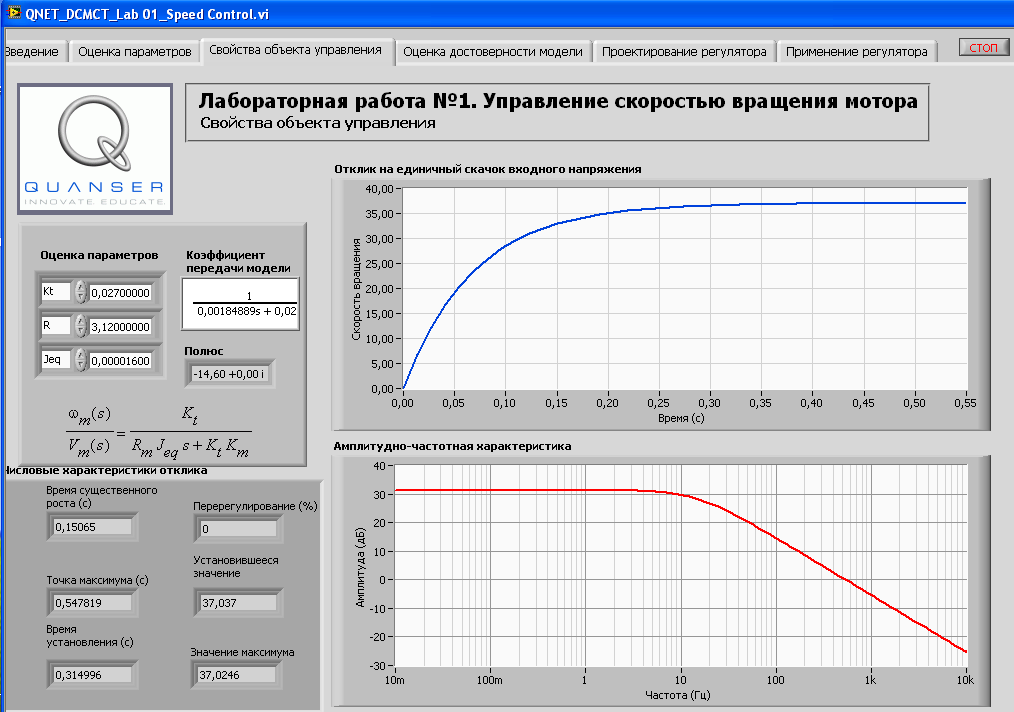
\includegraphics[scale=1.6]{response}
		\caption{Свойства объекта управления, как линейного динамического звена}
	\end{figure}
\end{center}
\begin{center}
	\begin{figure}
		\centering
		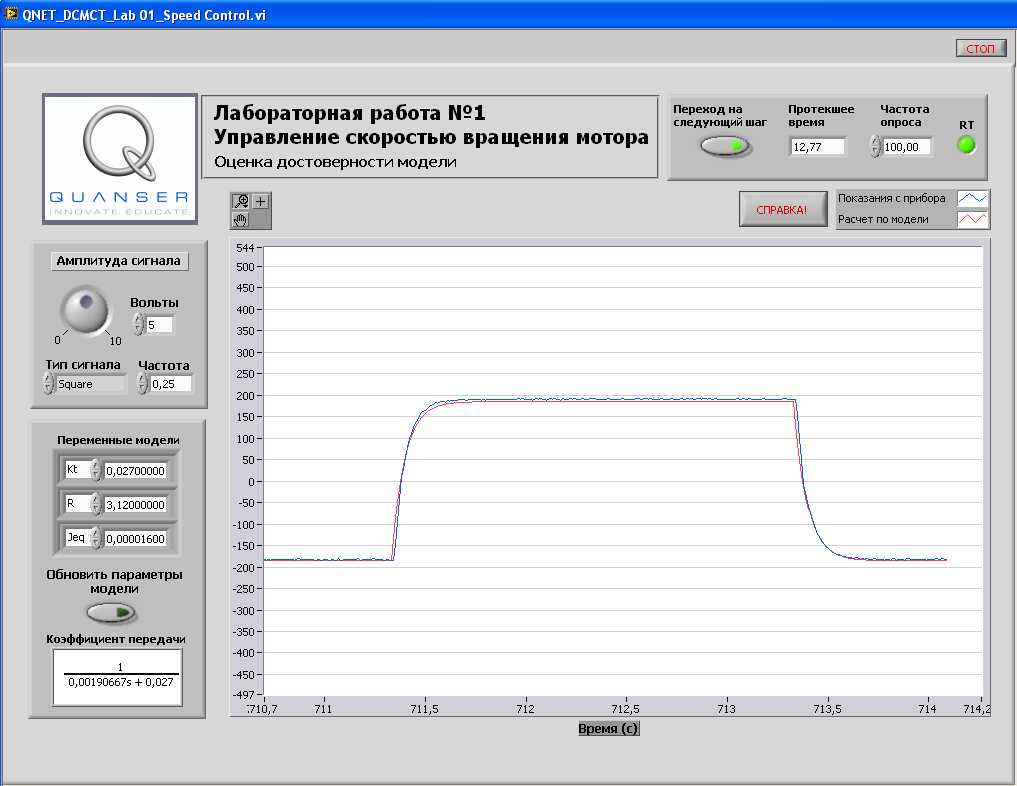
\includegraphics[scale=1.6]{square}
		\caption{Оценка достоверности построенной модели (отклик на тип сигнала Square)}
		\centering
		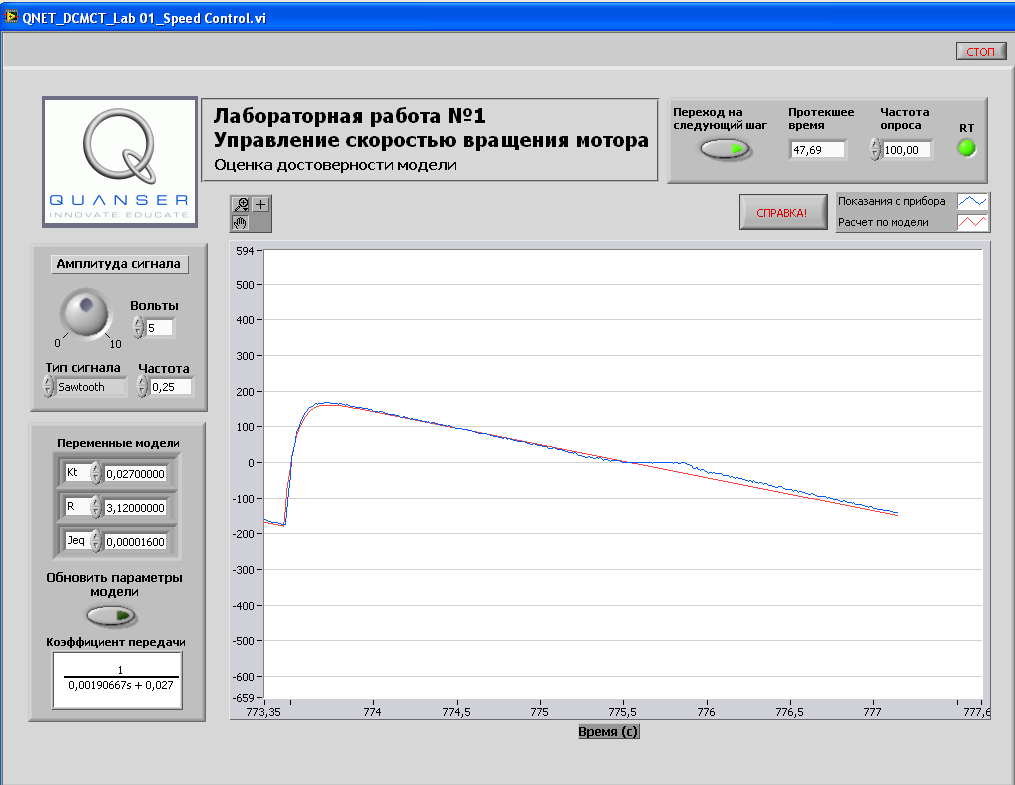
\includegraphics[scale=1.6]{sawtooth}
		\caption{Оценка достоверности построенной модели (отклик на тип сигнала Sawtooth)}
		\end{figure}
\end{center}
\begin{center}
	\begin{figure}
		\centering
		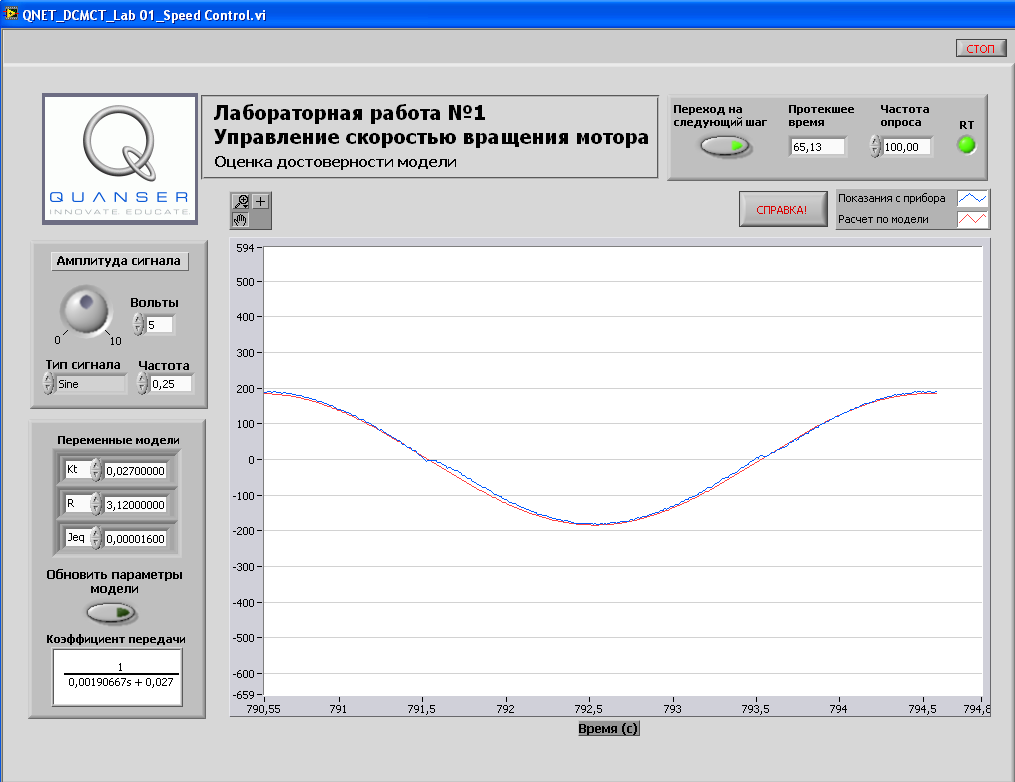
\includegraphics[scale=1.6]{sine}
		\caption{Оценка достоверности построенной модели (отклик на тип сигнала Sine)}
	\end{figure}
\end{center}
\vfill
\newpage


\section*{Построение регулятора скорости вращения}
\addcontentsline{toc}{section}{Построение регулятора скорости вращения}
\paragraph{}
Для управления электромотором необходимо построить
систему регулирования, на вход которой подавалась бы
требуемая скорость вращения $\omega^*(t)$. С помощью тахометра
можно измерить реальную скорость вращения $\omega(t)$ и
определить величину ее отклонения от заданной.
\paragraph{}
Будем использовать так называемый пропорционально-моторы используются повсеместно: в
интегральный регулятор (ПИ-моторы используются повсеместно: врегулятор), формирующий по этому отклонению значение входного напряжения на электромотор:
$V_m = K_p(\omega^*(t) - \omega(t))+K_t\int\limits_0^t(\omega^*(t) - \omega(t))dt$\hfill\break
\paragraph{}
Подавая на вход электромотора напряжение, зависящее от
величины ошибки регулирования, мы замыкаем систему
обратной связью.Проведём исследование полученной замкнутой системы.
Задача состоит в том, чтобы подобрать значения
коэффициентов $K_p$ и $K_i$, при которых выполняются следующие условия:
\begin{enumerate}
	\item время достижения максимума не превышает 0.15 секунд;
	\item перерегулирование (превышение реальной скорости над заданной) по значению составляет не более 5\%;
	\item время установления не превышает 0.25 секунд;
	\item установившаяся статическая ошибка должна быть равна 0\%.
\end{enumerate}
\paragraph{}
Будем изменять значения коэффициентов K p и K i учитывая
специфику их влияния на систему, а именно:
\begin{itemize}
	\item \textit{Пропорциональная} составляющая вырабатывает выходной
сигнал, противодействующий отклонению регулируемой
величины от заданного значения, наблюдаемому в данный
момент времени. Он тем больше, чем больше это отклонение.
Если входной сигнал равен заданному значению, то выходной
равен нулю. Однако при использовании только
пропорционального регулятора значение регулируемой
величины никогда не стабилизируется на заданном
значении. Существует так называемая статическая ошибка,
которая равна такому отклонению регулируемой величины,
которое обеспечивает выходной сигнал, стабилизирующий
выходную величину именно на этом значении.
\item \textit{Интегрирующая} составляющая пропорциональна интегралу
по времени от отклонения регулируемой величины. Еёиспользуют для устранения статической ошибки. Она
позволяет регулятору со временем учесть статическую
ошибку.
\end{itemize}
\paragraph{}
Полученные результаты занесем в таблицу.
\begin{table}
	
	\label{tab:3}

	\begin{center}
		\begin{tabular}{|c|c|C{2.3cm}|c|C{3cm}|C{3cm}|}
			 \hline
			 $K_p$ & $K_i$ & Точка первого макисмума & Перерегулирование(\%) & 
			 Время установления(c) & Установившаяся статическая ошибка(\%)\\
			 \hline
			 0.00 & 0.05 & 1.030 & 0.00 & 2.187 & 0.00\\
			 0.03 & 0.05 & 1.696 & 0.00 & 4.237 & 0.00\\
			 0.05 & 0.05 & 1.863 & 0.00 & 5.340 & 0.00\\
			 0.08 & 0.05 & 1.908 & 0.00 & 6.784 & 0.00\\
			 0.10 & 0.05 & 1.838 & 0.00 & 7.644 & 0.00\\
			 0.05 & 0.00 & 0.052 & 0.00 & 0.108 & 34.83\\
			 0.05 & 0.50 & 0.128 & 0.00 & 0.406 & 0.00\\
			 0.05 & 0.75 & 0.081 & 0.00 & 0.161 & 0.00\\
			 0.05 & 1.00 & 0.056 & 2.42 & 0.226 & 0.00\\
			 \hline
		\end{tabular}
	\end{center}
	\caption{Влияние параметров регулятора на характеристики переходного процесса}
\end{table}
\paragraph{}
Результирующие значения параметров регулятора, при
которых достигается выполнение всех естественных условий:
\begin{itemize}
	\item $K_p$ = 0.04 В/рад
	\item $K_i$ = 0.7 В/(рад$\cdot$с)
	\item Время достижения максимума = 0.088 с.
	\item Перерегулирование = 0.919\%
	\item Время установления = 0.143 с.
	\item Установившаяся ошибка = 0\%
\end{itemize}
\vfill
\paragraph{}
Результат управления можно увидеть на Рис.7-10. По данным графикам можно убедиться, что значения
коэффициентов $K_p$ и $K_i$ пропорциональной и интегральной
составляющих управления на панели «Параметры
регулятора» отвечают рассматриваемым ранее требованиям
на управление.
\vfill
\begin{center}
	\begin{figure}
		\centering
		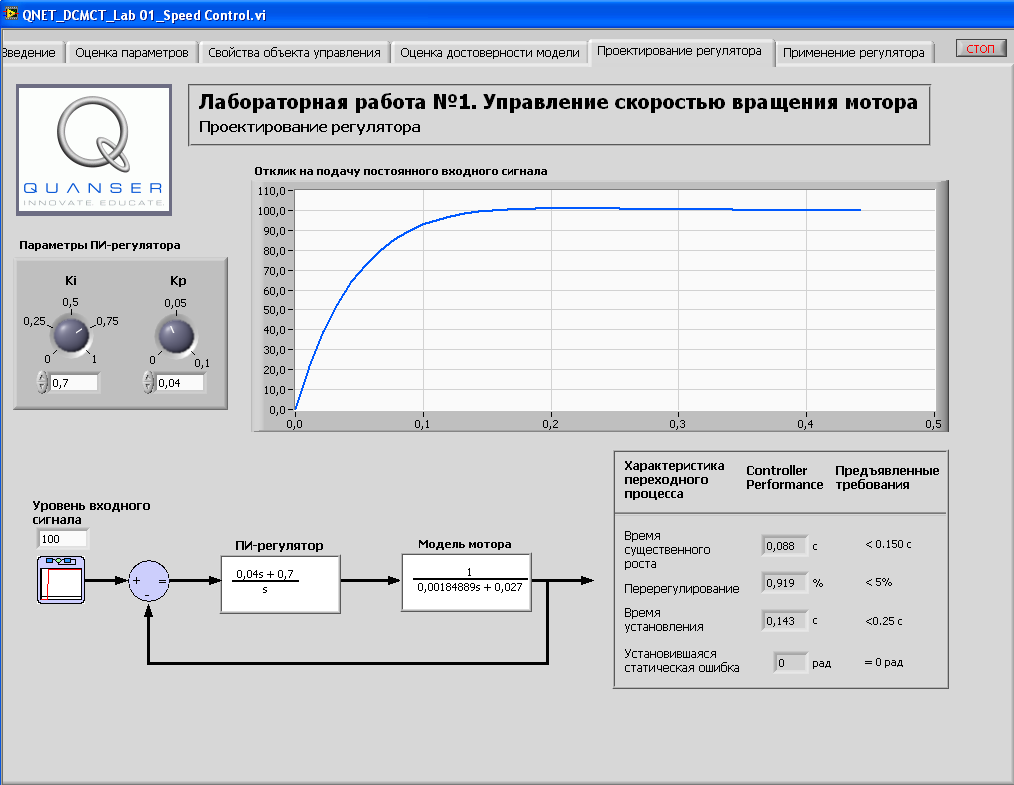
\includegraphics[scale=1.6]{control_response}
		\caption{Отклик на подачу постоянного входного сигнала при результирующих значениях параметров регулятора}
		\hfill\break
		\centering
		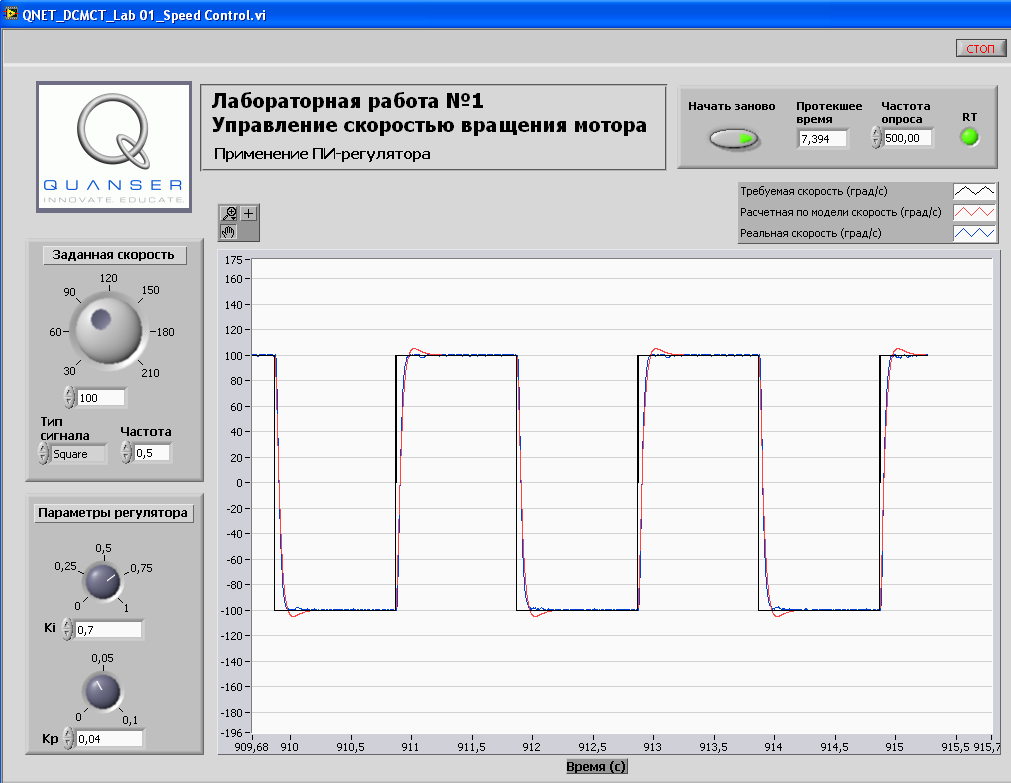
\includegraphics[scale=1.6]{control_square}
		\caption{Поведение функции отклика (тип входного сигнала Square) при результирующих значениях параметров регулятора}
	\end{figure}
\end{center}
\vfill
\begin{center}
	\begin{figure}
		\centering
		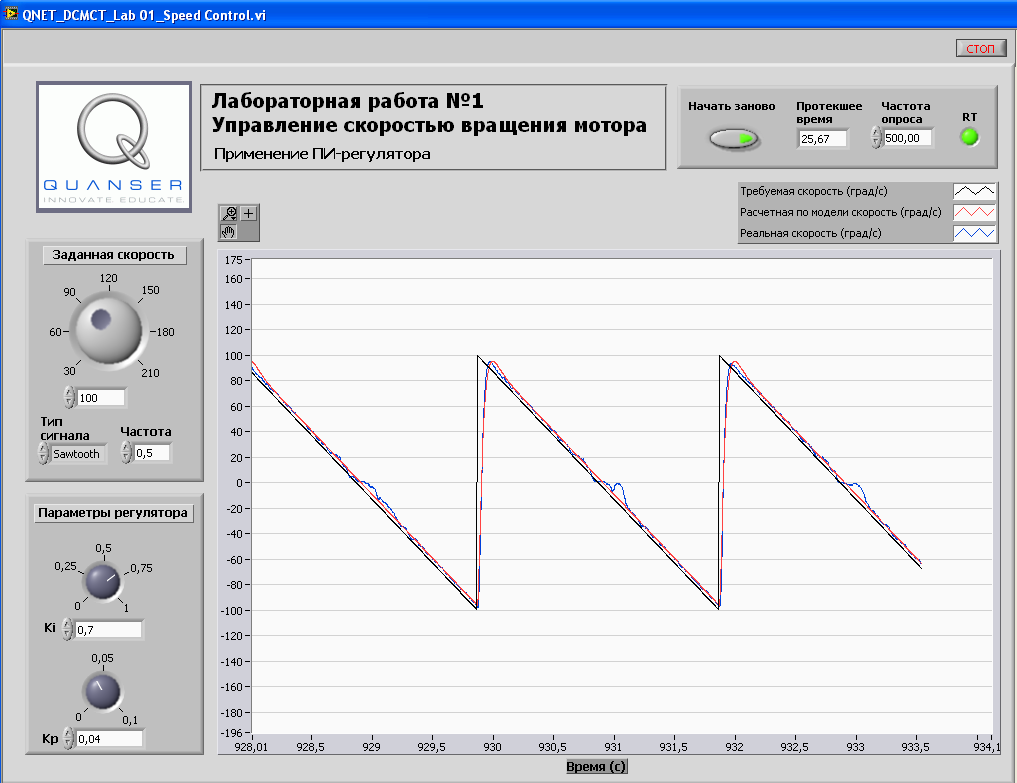
\includegraphics[scale=1.6]{control_sawtooth}
		\caption{Поведение функции отклика (тип входного сигнала Sawtooth) при результирующих значениях параметров регулятора}
		\hfill\break
		\centering
		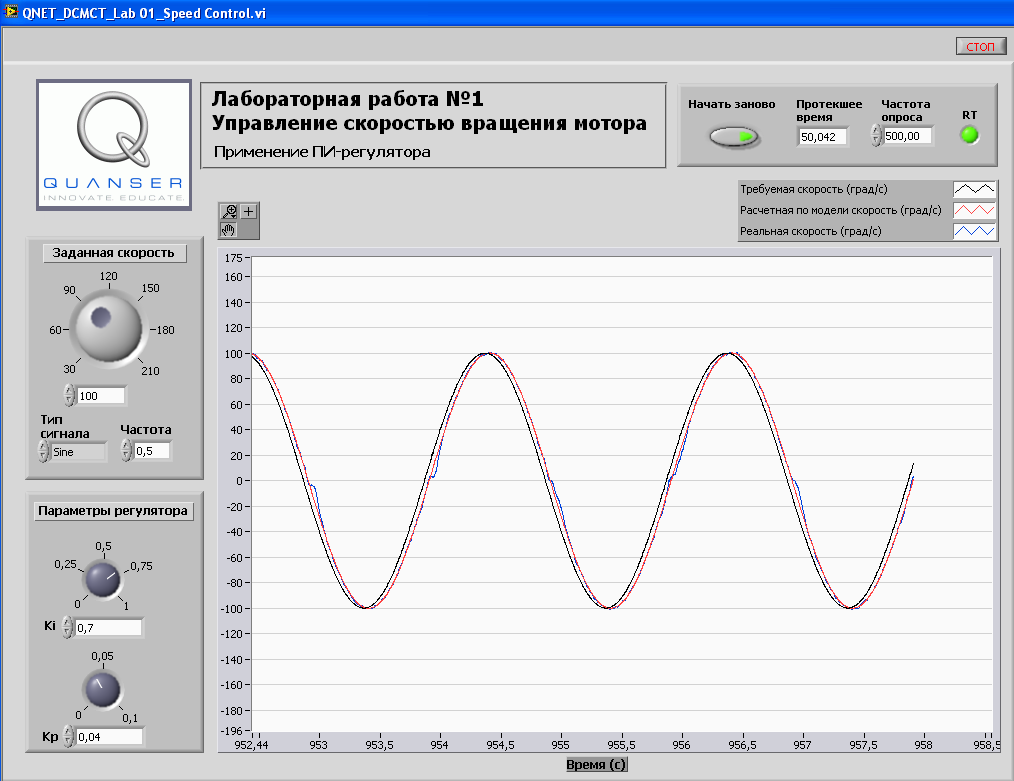
\includegraphics[scale=1.6]{control_sine}
		\caption{Поведение функции отклика (тип входного сигнала Sine) при результирующих значениях параметров регулятора}
	\end{figure}
\end{center}
\vfill
\newpage




\section*{Заключение}
\addcontentsline{toc}{section}{Заключение}
\paragraph{}
В рамках лабораторной работы были рассмотрены
физическая и электрическая модели DC-моторы используются повсеместно: вмотора. Построена
математическая модель. Далее была произведена
идентификация параметров математической модели объекта
на основе изучения реального поведения физического DC-моторы используются повсеместно: в
мотора. На основе полученной модели и вычисленных
параметров была построена система регулирования.
Параметры для ПИ-моторы используются повсеместно: врегулятора были экспериментально
подобраны с помощью исследования поведения реального
объекта и сопоставления результатов с поведением
математической модели.Полученная модель и ПИ-моторы используются повсеместно: врегулятор были использованы для
решения задачи поддержания заданного закона изменения
скорости вращения на реальном DC-моторы используются повсеместно: вмоторе. В итоге была
построена замкнутая система регулирования, которая
удовлетворяет заранее заданным ограничениям на
характеристики функции отклика (такие как точка первого
максимума, перерегулирование, время установления,
установившаяся статическая ошибка).\hfill\break
\vfill
\newpage









\section*{Литература}
\addcontentsline{toc}{section}{Литература}
\paragraph{}
Городецкий С.Ю., Бирюков Р.С., Кустикова В.Д.
КОМПЬЮТЕРНОЕ УПРАВЛЕНИЕ УГЛОВЫМ ПОЛОЖЕНИЕМ И
СКОРОСТЬЮ ВРАЩЕНИЯ ВАЛА ЭЛЕКТРОМОТОРА :
Практикум. – Нижний Новгород: Нижегородский
госуниверситет, 2008. – 50 с.
\newline
\newline
Неймарк Ю.И. Динамические системы и управляемые
процессы. – М.: Наука, 1978. – 336 с.
\newline
\newline


\vfill
\end{document}
